\chapter*[INTRODUÇÃO]{INTRODUÇÃO}
\addcontentsline{toc}{chapter}{INTRODUÇÃO}
\label{cap:Introducao}

 Atualmente, os smartphones são itens indispensáveis à vida em sociedade, já que possuem diversas funcionalidades que facilitam tarefas do cotidiano, como acessar internet, tirar fotos, encontrar lugares, etc. Dentre tais funcionalidades, \citeonline[p.~12]{marcarini_utfpr_2015} afirma que os dispositivos móveis com funcionalidade GPS são provavelmente a espécie de aparelhos eletrônicos com o maior crescimento nos últimos anos. Em razão disto o trabalho em questão propõe, a extensão da plataforma web já existente denominado Cidadão do Vale para aplicativo smartphone, que viabilizará uma parceria entre a prefeitura de Almenara-MG e os cidadões, através da coleta de informações precisas sobre as questões urbanas da cidade de Almenara, e também do seu contexto regional.  
 
 A plataforma Cidadão do Vale é uma configuração do framework ClickOnMap implementada em 2017 no IFNMG-Almenara em parceria com a Prefeitura Municipal, que permite o envio de informação sobre a existência de problemas relacionados à infraestrutura urbana. Desde o início do seu funcionamento, a plataforma contou com mais de mil contribuições públicas que, entre outros, revelou o perfil e distribuição espacial das principais reclamações, e apresentou-se como alternativa viável à gestão urbana da cidade.
 
 Soluções como a em curso compõem um fenômeno multidimensional associado a um novo paradigma tecnológico de circulação de informações. Este novo padrão ocorre por meio da coleta de informações voluntária dos cidadãos, este conceito é denominado Informação Geográfica Voluntária (VGI)\footnote{Em inglês, Voluntereed Geographic Information.}; \citeonline[p.~vii]{costa_enriquecimento_2018} define o VGI como "um tipo de informação com posicionamento geográfico e que é coletada e/ou compartilhada voluntariamente pelos usuários por meio da Internet".

 É inegável que a internet se tornou uma das principais fontes de acesso à informação global, e o uso de aplicativos moveis já são tendência em tecnologia no varejo. \citeonline{agencia_ibge_noticias2018}, mostra que o celular é o aparelho mais utilizado para a acessar à Internet (97,2\%) no total, o smartphone esta presenta em 46,7 milhões dos domicílios, 38,6\% o utiliza como única forma de acesso a internet, apesar de encontra-se presente em mais da metade (57,8\%) o computador fica na segundo posição com apenas 2,3\% de uso, o terceiro lugar ficou para o tablet (17,8\%), seguido pela televisão (11,7\%) e outros equipamentos (1,3\%), houveram variações em grandes regiões como mostra a Figura 1. Tais informações revelam a importância dos aplicativos para dispositivos móveis como meio de comunicação da população.
 \begin{figure}[H]
 	\centering
 	\caption{Percentual de domicílios brasileiros com acesso à Internet, segundo o equipamento utilizado.(2016)}
 	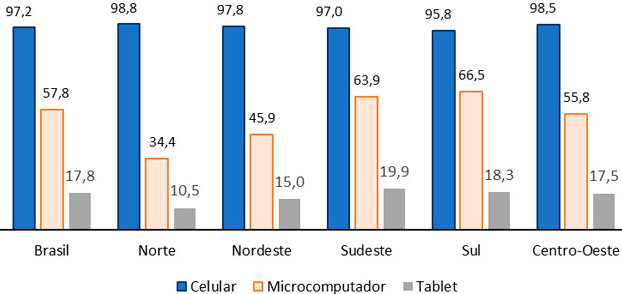
\includegraphics[width=0.6\linewidth]{Imagens/grafico} 	
	\legend{Fonte: \citeonline{agencia_ibge_noticias2018}}
 \end{figure}
 
  Ambientes urbanos são os espaços de produção e reprodução da vida social e onde as oportunidades de trabalho, educação, saúde, cultura, lazer e todas outras dimensões da vida cotidiana se concentram. O \citeonline[p.~19]{IBGEIBGE2011} define este termo como, "área legalmente definida como urbana, que se caracteriza por construções, arruamentos e intensa ocupação humana". Estes espaços vem  aumentando constantemente, como podemos ver na a Figura 2 abaixo. 
  \begin{figure}[H]
	\centering
 	\caption{Grau de urbanização, segundo as Grandes Regiões 1991/2010.} 
 	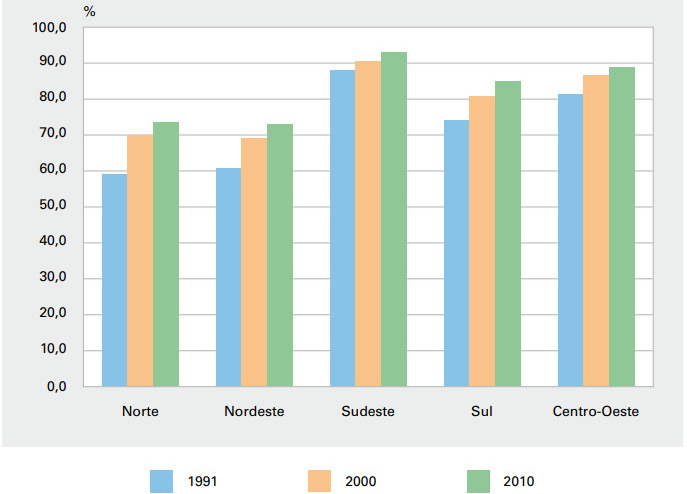
\includegraphics[width=0.6\linewidth]{Imagens/grafico2}		
	\legend{Fonte: \citeonline[p.~46]{IBGEIBGE2011} }
 \end{figure}  

 \citeonline[p.~7]{hyller_bandeira_dutra_cidadao_2018} realizou um levantamentos por meio de conversas informais com moradores, nas quais revelaram que são comuns as reivindicações da população em relação à resolução de problemas, utilizando canais de comunicação como a rádio local, o telefone da prefeitura, e mídias sociais como Facebook e WhatsApp. A variedade de meios de comunicação, embora conveniente, dificulta o gerenciamento e a gestão das informações fornecidas. 

 Desta maneira, uma aplicação de um sistema para dispositivos moveis como o Cidadão do Vale configura-se como uma alternativa via sistema informacional que possibilita a centralização, organização e georreferenciamento das informações. O emprego de um sistema mobile, associado aos conceitos de VGI, facilita a comunicação entre as pessoas e a gestão municipal ao proporcionar um veículo de comunicação com dados objetivos, disposição das informações de forma pública, com possibilidade, inclusive, de pesquisas sobre a situação do município.

\section*{Objetivo Geral} 
Facilitar o gerenciamento dos problemas na infraestrutura em Almenara – MG, por meio do desenvolvimento de um sistema Android baseado no Cidadão do Vale.
	
\section*{Objetivos Específicos}

\begin{flushleft}
	Como objetivos específicos pretende-se:
\end{flushleft}
\begin{itemize}
	\item Levantar requisitos do sistema web Cidadão do Vale;
	\item Desenvolver um aplicativo para dispositivos móveis com base no Cidadão do Vale;
	\item Atualizar o mapeamento dos problemas relacionados à infraestrutura urbana de Almenara;
	\item Alertar o poder público dos problemas na infraestrutura de Almenara – MG;
\end{itemize}

\section*{Justificativa}
A proposta justifica-se pela possibilidade de eliminação da necessidade de pesquisas de data fixa, onerosas ao poder público, já que o sistema web viabiliza o fluxo continuo de informações e, consequentemente, de resoluções. A manutenção de um canal público capaz de centralizar as informações sobre a infraestrutura urbana em ambiente WebGIS e a visualização integrada território almenarense poderá auxiliar no processo de tomada de decisões e facilitar o diálogo entre a população e a gestão pública. Tais iniciativas geram impactos positivos sobre o orçamento público e democratizam o acesso a informação sobre a gestão do espaço urbano, e reafirmam o compromisso do IFNMG previsto na Lei nº. 11.892/08 \citeonline{LILDS2008}, de “orientar sua oferta formativa em benefício da consolidação e fortalecimento dos arranjos produtivos, sociais e culturais locais, identificados com base no mapeamento das potencialidades de desenvolvimento socioeconômico e cultural no âmbito de atuação do Instituto Federal”.

\section*{Resultados Esperados}
Espera-se que o este trabalho continue suas contribuições para o desenvolvimento urbano de Almenara e estreite as relações entre o IFNMG e a gestão municipal. Além disso, a expectativa é de que o aplicativo desenvolvido aproxime a população municipal da gestão pública por meio de suas contribuições online medida. A transparência e o diálogo são meios fundamentais para o alcance da cidadania plena.

